\chapter{Focus Projection}
\label{chapter10-4}
\setcounter{enums}{0}


Focus projection\is{focus projection} occurs when the meaning of \isi{focus}
that is associated with specifically marked words is spread a larger
phrase to which the word belongs.  In previous research, it has been
said that a typical focus domain in a sentence must contain at least
one accented word, which functions as the core of focus meaning. That
implies that focus projection can be seen to be related to how
F(ocus)-marking (normally realized with a specific pattern of
prosody,\is{prosody} such as the A-accent (H*) in \ili{English}) co-operates
with information structure meanings.\is{A-accent} The fundamentals of
focus projection, suggested by \citet{selkirk:84,selkirk:95} and
\citet{buring:06}, are summarized as follows.  These definitions
remain true when observing English in which prosody is mainly
responsible for expressing focus.



\myexe{\eenumsentence{\label{def:focus-projection:ch10-4}
\item{Basic Focus Rule: An accented word is F-marked.}
\item{Focus of a sentence: An F-marked constituent is not dominated by
  any other F-marked constituent.}
\item{Focus Projection: either (i) F-marking of the head of a phrase
  licenses F-marking of the phrase, or (or both) (ii) F-marking of an
  internal argument of a head licenses the F-marking of the
  head. \citep[p.\ 322--323]{buring:06}}}}



This chapter lays the groundwork for how an analysis based on
\isi{ICONS} (Individual CONStraints)\is{individual constraints} and
MKG (MarKinG)\is{MKG} could eventually support a deeper study of focus
projection.\is{HPSG} A large number of HPSG-based studies on
information structure are particularly concerned with \isi{focus}
projection, mostly based on the Focus Projection Principle as
presented in \myref{def:focus-projection:ch10-4}.  The previous
studies have three points in common, but these points need to be taken
into account in the context of creation of a computational model:
First, they provide multiple parse trees for a single sentence in
which \isi{focus projection} may occur.  The first section
(\myS{10:sec:parse-trees}) provides a counterargument to this strategy
in representation.  Second, previous studies claim that assignment of
focus-marking accent plays an important role in calculating the extent
of focus domain (\myS{10:sec:f-marking}).\is{focus projection} Third,
distinctions between grammatical relations, such as peripheral \vs
non-peripheral, head \vs non-head, are critically used in constraining
focus projection (\myS{10-4:sec:grammatical}).\is{periphery} The last
section (\myS{10-4:sec:analysis}) formulates an illustrative analysis
of a single sentence in which we find that focus projection occurs.










\section{Parse Trees}
\label{10:sec:parse-trees}

Most previous approaches in the HPSG-based\is{HPSG} study on
information structure provide multiple parse trees.\is{HPSG} In fact,
a sentence that potentially involves \isi{focus} projection sounds ambiguous
in and of itself. For example, \myref{exe:fp:multiple} may have at
least three parse trees following the previous approaches.\is{focus
  projection}

\myexe{\enumsentence{\label{exe:fp:multiple}
[$_{f}$ Kim [$_{f}$ gives Lee [$_{f}$ a \textsc{book}]]]. 
}}


\noindent From the perspective that a single sentence may have
multiple readings, following this method may not seem so odd. However,
this kind of approach does not work well in the context of
computational processing.  The issue baring the most concern would be
when multiple parse trees for a single sentence can have an adverse
effect on system performance.  A large number of parse trees decreases
speed while an increase in ambiguity decreases accuracy, both
detrimental to the system's goals. That is, several external modules
that enhance feasibility of computational grammars (e.g.\ reranking
model) do not perform actively with such a large number of
intermediate results. Thus, I argue that a single parse tree that
potentially transmits the complete meanings that the sentence may
convey should necessarily be provided.  The main mechanism to
facilitate this flexibility is \isi{underspecification}.


\section{F(ocus)-marking}
\label{10:sec:f-marking}


F-marking, which crucially contributes to formation of \isi{focus projection}, 
has been presumed to be closely associated with
prosody,\is{prosody} as shown in
(\ref{def:focus-projection:ch10-4}a). That is to say, in previous
literature, a set of specific accents (e.g.\ the A-accent in
\ili{English})\is{A-accent} has been considered tantamount to F-marking.
However, it is my position that bearing a specific accent is not a
necessary condition, but a sufficient condition for F-marking:
F-marking does not necessarily depend on whether the word is accented
or not. Across languages, there are several examples in which focus
projection is triggered by non-prosodic features.


Building on the phonological rules provided in
\myref{avm:bildhauer:rules:ch10-3} (already presented in
\myS{8:sec:phonology}),\is{focus prominence} the \isi{focus} prominence rule
that \citet{bildhauer:07} derives is constrained as represented in
\myref{avm:bildhauer:rules:ch10-3}. The constraints signify that the
focused constituent has to contain the Designated Terminal Element
(DTE) on the level of phonological UTterance (UT). (In the following
rules, PHP is short for PHonological Phrase, IP for Intonational
Phrase, RE for Right Edge, PA for Pitch Accent, and BD for BounDary
tone.)


\myexe{\eenumsentence{\label{avm:bildhauer:rules:ch10-3}
\item\evnup{{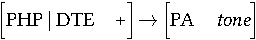
\includegraphics{pdf/php-plus.pdf}}}
\item\evnup{{
\includegraphics{pdf/php-minus.pdf}}}
\item\evnup{{
\includegraphics{pdf/ip-plus.pdf}}}
\item\evnup{{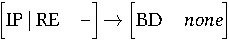
\includegraphics{pdf/ip-minus.pdf}}}}}



\myexe{\enumsentence{\label{avm:bildhauer:focus-prominence}\evnup{
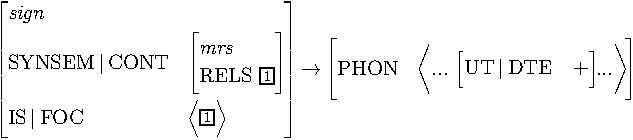
\includegraphics{pdf/focus-prominence-bildhauer.pdf}}}}


\noindent \citeauthor{bildhauer:07} claims that the schematic AVM
\myref{avm:bildhauer:focus-prominence} can be presumably applied to
most human languages in which \isi{focus} in marked by means of prosody.
Furthermore, it may have a subtype which places a more precise
constraint.\is{focus prominence} For instance, given that focus
prominence in \ili{Spanish} has a strong tendency to fall on the last
prosodic word in the PHON list of a focused sign,
\myref{avm:bildhauer:focus-prominence} can be altered into
\myref{avm:bildhauer:focus-prominence-spa} in Spanish
(Ibid.\ p.\ 191).

\myexe{\enumsentence{\label{avm:bildhauer:focus-prominence-spa}\evnup{
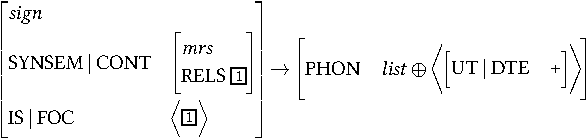
\includegraphics{pdf/focus-prominence-spa.pdf}}}}


\noindent One of the greater strengths that this formalism provides
may very well be that the relation between \isi{focus} and prosodic
prominence is restricted in a fairly straightforward manner as shown
in \myref{avm:bildhauer:focus-prominence}. In addition, it is a
significant endeavor to the HPSG framework to look into how various
phonological layers interact with each other in phases and end up with
focus projection.\is{focus projection}\is{HPSG}


However, these AVMs are viewed differently with the current model.  I
propose to argue that F-marking is most relevant to marking
information structure.\is{prosody} In \ili{English}, prosody has a
relatively straightforward relationship to information structure
marking. However, this does not hold necessarily true in other
languages.  Instead, I argue that F-marking needs to be represented as
MKG{$\mid$}FC in the current formalistic framework. In other words,
\mbox{[MKG{$\mid$}FC +]} indicates that the word (or the phrase) is
F(ocus)-marked.\is{MKG} As the name itself implies, F-marking is a
matter of markedness, rather than a meaning. In brief, F-marking,
which triggers the spread of \isi{focus}, has to be specified as a feature
of MKG under CAT. There several reasons for this argument, which are
discussed in the following subsections.



\subsection{Usage of MRS}
\label{8:ssec:usage}


First of all,\is{MRS} the two AVMs
\myref{avm:bildhauer:focus-prominence} and
\myref{avm:bildhauer:focus-prominence-spa} proposed by
\citet{bildhauer:07} have an inconsistency with the \isi{DELPH-IN}
formalism that the present study relies on.  In the \isi{DELPH-IN}
formalism of HPSG,\is{HPSG} we cannot search a specific element
included in a list unless we create pointers into RELS (like ICONS-KEY
in the present work).\is{ICONS-KEY}






\subsection{Languages without Focus Prosody}
\label{8:ssec:no-prosodic}


Second, as presented in Chapter~\ref{chapter4}
(\myS{4:sec:prosody}),\is{prosody} some languages do not use prosody
in expressing \isi{focus} (e.g.\ \ili{Yucatec Maya} \citep{kugler:etal:07},
\ili{Akan} \citep{drubig:03}, and \ili{Catalan}
\citep{engdahl:vallduvi:96}).  Besides, in \ili{Hausa}, prosodic
prominence is disallowed for focus \textit{in situ}
\citep{hartmann:zimmermann:07,buring:10} \mypage{exe:hau}.\is{focus
  projection} If focus projection always occurred by means of prosody,
there could be no focus projection in these languages. Yet, it can be
understood that focus projection seems to be a universal phenomenon in
human language \citep{buring:06}.




\subsection{Lexical Markers}
\label{8:ssec:comment-scope}

Finally and most importantly, some languages make use of lexical
markers to invoke focus projection.\is{focus projection} Some previous
studies regard these lexical items as comment markers or scope
markers.  For instance, \ili{Korean} employs \textit{man} `only', and
this lexical item contributes to extension of focus
meaning,\is{prosody} although a specific pattern of prosody may or may
not occur when an element is focused \citep{choe:02}.  Similarly,
\textit{ba} in \ili{Abma} \citep{schneider:09} and \textit{sh\`{i}} in
Mandarin \ili{Chinese} \citep{prince:12} function to extend \isi{focus}
meaning into the larger constituents.  Thus, the main component
responsible for the spreading of focus meaning in these specific types
of languages is not necessarily prosody.



\section{Grammatical Relations}
\label{10-4:sec:grammatical}

In previous HPSG-based studies,\is{HPSG} ARG-ST or a linear
arrangement of dependents of verbs play a crucial role in identifying
which phrases are projected from a F(ocus)-marked word.\is{focus
  projection} \citet{engdahl:vallduvi:96} claim that focus projection
can be licensed if and only if the most oblique argument of the
phrase's head is F-marked. Their INFO-STRUCT instantiation principles
(for \ili{English}) are as follows.\is{narrow focus}\is{wide focus}


\myexe{\eenumsentence{\label{def:engdahl:vallduvi:96}
\item{Either if a DAUGHTER's INFO-STRUCT is instantiated, then the
  mother inherits this instantiation (for narrow foci, links and
  tails),}
\item{or if the most oblique DAUGHTER's FOCUS is
  instantiated, then the FOCUS of the mother is the sign itself (wide
  focus). \citep[p.\ 12]{engdahl:vallduvi:96}}}}




\noindent \citet{dekuthy:00} provides a different argument with
reference to the linear order of constituents; \isi{focus} projection can
happen if and only if the rightmost daughter is accented. Since the
rightmost daughter is not always an oblique argument,\is{focus
  projection} \citeauthor{dekuthy:00}'s focus projection rules are not
concurrent with the claim made by \citeauthor{engdahl:vallduvi:96}.
The main point that \citet{chung:etal:03} propose is that ARG-ST is
the locus in which focus projection occurs, which is largely in line
with \citeauthor{engdahl:vallduvi:96}, but there are some differences.
They add two more factors into the formation of focus projection.  One
includes modification and coordination. The focus that a modifier
bears can hardly spread into its modificand and the larger phrase, and
none of the operands in coordination (i.e.\ non-headed phrases) can
project focus.\footnote{A counterexample to this generaliztion is provided in
  \citet[326f.]{buring:06}: ``I know that John drove Mary's red
  convertible. But what did Bill drive? -- He drove her
  [$_{f}$\textsc{blue} convertible].''  To my understanding, this
  counterexample is relevant to contrastive focus, given that the
  correction test is applied (see
  \myS{3:ssec:tests-contrast} \mypage{3:ssec:tests-contrast}). The
  distinction between \isi{contrastive focus} and \isi{non-contrastive focus} with
  respect to focus projection is one of the major further topics.}
The other is agentivity. If the focus value of the non-agentive lowest
ranking argument is instantiated in its local position, then focus
projection can take place. \citet{bildhauer:07} is another endeavor to
show how focus projection can be dealt with within HPSG
formalism.\is{HPSG} \citeauthor{bildhauer:07} points out various
problems with previous studies: First, looking at obliqueness would
sometimes be too rigorous or sometimes too loose to identify how the
focus domain is built up. Second, the previous approaches are
language-specific, and thereby may not be straightforwardly applied to
other languages.









There are potentially (at least) six possibilities in spreading of
\isi{focus} meaning in \ili{English}. For instance, a ditransitive sentence
\textit{Kim sent Lee a big book yesterday.} consists of six components
as shown in (\ref{exe:8poss}).



\myexe{\enumsentence{\label{exe:8poss}
\evnup{\begin{tabular}[h]{lllll}
Kim & sent & Lee\\
(i) subject & (ii) verb & (iii) non-peripheral argument\\
\end{tabular}}
\newline
\evnup{\begin{tabular}[h]{lll@{}l@{}l}
a & big & book & yesterday.\\
  & (iv) NP modification \xspace \xspace & (v)  peripheral argument \xspace \xspace & (vi) VP modification\\
\end{tabular}}}}




First, \isi{focus} associated with (i) subjects cannot be projected into the
larger phrase \citep{chung:etal:03}. Although the subject in
(\ref{exe:8poss}) bears the A-accent (i.e.\ \textsc{Kim}), the whole
sentence cannot be in the focus domain.\is{A-accent} In other words, a
Q/A pair (\ref{exe:8poss:1}Q2-A2) sounds infelicitous, whereas
(\ref{exe:8poss:1}A1) sounds good as an appropriate reply to
(\ref{exe:8poss:1}Q1).

\myexe{\enumsentence{\toplabel{exe:8poss:1}
\begin{tabular}[t]{ll}
Q1: & {Who sent Lee a big book yesterday?}\\
A1:  & {[$_{f} $\textsc{Kim}] sent Lee a big book yesterday.}\\
Q2: & {What happened?}\\
A2:  & {\#[$_{f} $\textsc{Kim} sent Lee a big book yesterday.].}\\
\end{tabular}}}

\noindent This is in accordance with the proposal of
\citet{selkirk:84,selkirk:95}. The subject is neither the head of the
sentence nor an internal argument of the main verb.  However, when the
subject is an internal argument, the focus on subjects can be
projected. The subjects of unaccusative verbs (e.g.\ \textit{die})
have been analyzed as not an external argument of the verbs, but an
internal argument. \citet{chung:etal:03} argue that whether the
subject is an internal argument of the verb or not assists in
identifying focus projection. Since unergative verbs, such as
\textit{ran} in (\ref{exe:8poss:1-1}b), take their subject as an
external argument, the focus cannot be projected from the
subject.\is{focus projection} In contrast, \textit{Tom} in
(\ref{exe:8poss:1-1}a) may act as the core of \isi{focus projection}, due to
the fact that the verb \textit{died} takes it as an internal argument.

\myexe{\enumsentence{\toplabel{exe:8poss:1-1}
\begin{tabular}[t]{ll}
a. & {[$_{f}$ \textsc{Tom} died].}\\
b. & {\#[$_{f}$ \textsc{Tom} ran]. \citep[p.\ 395]{chung:etal:03}}\\
\end{tabular}}}

Second, it has been said that \isi{focus} on (ii) verbs can be projected
into the larger phrases (e.g.\ VP and S), but \citet{gussenhoven:99}
argues that such a projection is incompatible with intuition.  That
is, the following Q/A pair does not sound natural to
\citeauthor{gussenhoven:99}. That is to say, the focus associated with
\textsc{sent} cannot be projected into the VP.



\myexe{\enumsentence{\toplabel{exe:8poss:2}
\begin{tabular}[t]{ll}
Q: & {What did she do?}\\
A: & {\#She \textsc{sent} a book to Mary.}\\
\end{tabular}}}


Third, distinction between (iii) non-peripheral argument and (v)
peripheral argument with respect to \isi{focus projection} has already been
the subject of in-depth research.  \citet{bresnan:71} argues that
focus projection in \ili{English} happens if and only if the A-accented word
is the peripheral argument.\is{A-accent}


\myexe{\enumsentence{\toplabel{exe:8poss:3}
\begin{tabular}[t]{ll}
a. & {The butler [$_{f}$ offered the president some \textsc{coffee}].}\\
b. & {*The butler [$_{f}$ offered the \textsc{president} some coffee].}\\
c. & {The butler offered [$_{f}$ the  \textsc{president} some coffee].} \\ 
   & \mbox{ } \mbox{ } \mbox{ } \mbox{ } \mbox{ } \mbox{ } 
\mbox{ } \mbox{ } \mbox{ } \mbox{ } \mbox{ } \mbox{ } 
\mbox{ } \mbox{ } \mbox{ } \mbox{ } \mbox{ } \mbox{ } 
\mbox{ } \mbox{ } \mbox{ } \mbox{ } \mbox{ } \mbox{ } 
\citep[p.\ 388]{chung:etal:03}\\
\end{tabular}}}


Fourth, modifiers (i.e.\ (iv) and (vi)) are less capable of extending
the \isi{focus} that they are associated with to their head phrases. Thus,
any head can hardly inherit a focus value from its adjunct.

In the following section, I narrow down the scope of analysis to the
distinction between (iii) non-peripheral argument and (v) peripheral
argument, and will address the full range of focus projection in
future research with deeper analysis.



\section{An Analysis}
\label{10-4:sec:analysis}

My investigation provides makes use of \isi{ICONS} and MKG.\is{focus
  projection}\is{MKG} They are used to place a restriction on
possibility of focus projection and to represent the meaning of a
sentence in which focus projection can occur into a single parse tree.


\subsection{Basic Data}
\label{10-4:ssec:basic}

A set of allosentences (i.e.\ close paraphrases which share
truth-conditions \citep{lambrecht:96}) is presented in
\myref{exe:lee:1},\is{truth-conditions} and the principle difference
among them is the position of the A-accent (marked as \textsc{small
  caps}).\is{A-accent} In other words, what is focused upon is
different in the different allosetences.

\myexe{\enumsentence{\toplabel{exe:lee:1}
\begin{tabular}[t]{ll}
a. & {\textsc{Kim} sent Lee the book.}\\
b. & {Kim \textsc{sent} Lee the book.}\\
c. & {Kim sent \textsc{Lee} the book.}\\
d. & {Kim sent Lee the \textsc{book}.}\\
\end{tabular}}}



According to \citet{bresnan:71}, among these allosetences, \isi{focus}
projection can happen only in (\ref{exe:lee:1}d): Only the most
peripheral argument can be the starting point of \isi{focus projection}. For
example, if a \textit{wh-}question requires an answer of
\tdl{all-focus} (``an absence of the relevant presuppositions''
\citep[p.\ 232]{lambrecht:96}), only the sentence in which the most
peripheral argument bears an focus-marking (e.g.\ the A-accent) sounds
felicitous,\is{A-accent} as exemplified in \myref{exe:lee:2}.\footnote{I would
  rather say ``focus-marked'' rather than ``accented'', because
  F(ocus)-marking does not necessarily mean prosodic marking as
  discussed before.}


\myexe{\enumsentence{\toplabel{exe:lee:2}
\begin{tabular}[t]{ll}
Q: & {What happened?}\\
A1: & {\#[$_{f}$ \textsc{Kim} sent Lee the book].}\\
A2: & {\#[$_{f}$ Kim \textsc{sent} Lee the book].}\\
A3: & {\#[$_{f}$ Kim sent \textsc{Lee} the book].}\\
A4: & {[$_{f}$ Kim sent Lee the \textsc{book}].}\\
A5: & {\#Kim sent [$_{f}$ Lee the \textsc{book}].}\\
\end{tabular}}}

\noindent In addition, there are two more restrictions on the
occurrence of focus projection: First, focus projection takes place
only when the syntactic head dominates the focus-marked element.  For
instance, focus cannot be projected in the way presented in
(\ref{exe:lee:2}A5) in which the verb \textit{sent} is not in the
focus domain.  Second, the focus-marked element should be included in
the focus domain. For instance, the followings in which the
focus-marked \textit{\textsc{book}} is out of the bracket are
ill-formed.

\myexe{\enumsentence{\label{exe:lee:4}
\begin{tabular}[t]{ll}
a. & {*[$_{f}$Kim] sent Lee the \textsc{book}.}\\
b. & {*[$_{f}$Kim sent]  Lee the \textsc{book}.}\\
c. & {*[$_{f}$Kim sent Lee] the \textsc{book}.}\\
d. & {*Kim [$_{f}$ sent] Lee the \textsc{book}.}\\
e. & {*Kim [$_{f}$ sent Lee] the \textsc{book}.}\\
f. & {*Kim sent [$_{f}$ Lee] the \textsc{book}.}\\
\end{tabular}}}


\subsection{Rules}
\label{10-4:ssec:Rules}


The present study follows the idea \citet{chung:etal:03} propose:
ARG-ST is the locus where \isi{focus} projection takes place.\is{focus
  projection} That means that the main constraint on the range of
spreading focus should be specified in the lexical structure of the
verb (i.e.\ \textit{sent} in (\ref{exe:lee:2}A4)). I introduce extra
lexical rules to manipulate the feature structure(s) under VAL for
constraining such a possibility of focus projection. That is, each
verbal entry has its own ARG-ST independent of focus marking, and one
extra verbal node is introduced at the lexical level when constructing
a parse tree. On the other hand, the lexical rules for calculating
focus projection refer to F-marking specified as a value of
MKG{$\mid$}FC of the dependents specified in the list of
VAL{$\mid$}COMPS (and VAL{$\mid$}SUBJ).\is{MKG}



I propose a ditransitive verbal entry \textit{send} used in
(\ref{exe:lee:2}A4)) takes \ensuremath{<}NP(\textsc{nom}),\is{focus projection}
NP(\textsc{acc}), NP(\textsc{acc})\ensuremath{>} (i.e.\ two elements
in COMPS) as its ARG-ST.\footnote{In the \isi{ERG} (English Resource
  Grammar, \citealt{flickinger:00}), a default form of \textit{send}
  is divided into several different types, mainly depending on
  specification of ARG-ST, such as `send\_v1', `send\_v2', etc.
 I follow this strategy of enumerating verbal entries.}  The basic
entry is conjugated into \textit{sent} by inflectional rules, and the
inflected element can be the daughter of the lexical rules that I
employ for computing focus projection. There are two rules to look at
the values in VAL{$\mid$}COMPS, as presented below.









\myexe{\eenumsentence{\label{avm:fp:rules}
\item\evnup{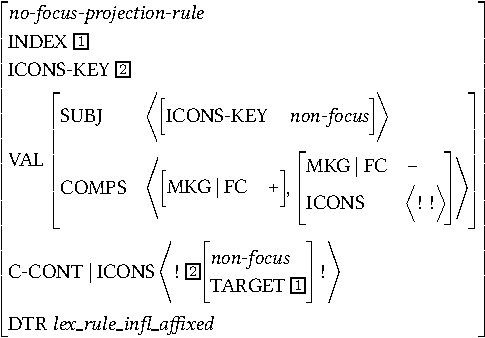
\includegraphics{pdf/fp-rule1.pdf}}
\item\evnup{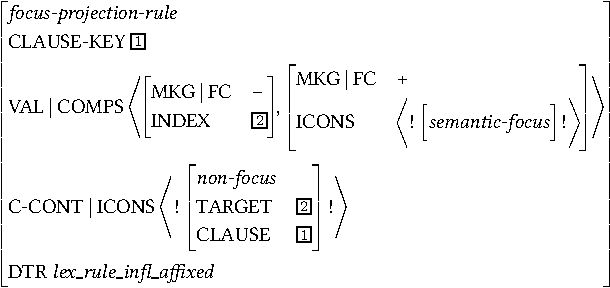
\includegraphics{pdf/fp-rule2.pdf}}}}

\noindent \tdl{No-focus-projection-rule} shown in
(\ref{avm:fp:rules}a) takes a non-focus-marked element as the last
component, while \tdl{focus-projection-rule} shown in
(\ref{avm:fp:rules}b) takes a focus-marked one. Focus projection in a
sentence whose main verb stems from \textit{send} can happen by using
only \tdl{focus-projection-rule}, and \tdl{no-focus-projection-rule}
predicts other sentences in which the most peripheral argument
(i.e.\ \textit{the book} in this case) introduces no \tdl{info-str}
value into ICONS.\is{periphery}\is{\textit{info-str}} Note that
\tdl{focus-projection-rule} requires one information structure value
(specified as \tdl{semantic-focus}) from the last element in
VAL{$\mid$}COMPS.\is{semantic focus}


For example, (\ref{exe:lee:5}a-b) are not compatible with each
other. When \textit{Lee} is A-accented (i.e.\ \textsc{Lee} with [FC
  +]), (\ref{avm:fp:rules}b) cannot take it as its
complement.\is{A-accent} (\ref{avm:fp:rules}a) can take \textsc{Lee} as its
complement, but (\ref{avm:fp:rules}a) prevents the A-accented
\textsc{book} with [FC +] from being the second complement.  In other
words, \textit{sent} in (\ref{exe:lee:5}a) is constrained by
(\ref{avm:fp:rules}a), while that in (\ref{exe:lee:5}b) is constrained
by (\ref{avm:fp:rules}b).



\myexe{\enumsentence{\toplabel{exe:lee:5}
\begin{tabular}[t]{ll}
a. & {Kim sent \textsc{Lee} the book.}\\
b. & {Kim sent Lee the \textsc{book}.}\\
\end{tabular}}}



\subsection{Representation}
\label{10-4:ssec:representation}


The primary motivation to use \isi{ICONS} with respect to \isi{focus}
projection is to provide only one single parse tree that covers all
potential meanings of \isi{focus projection}. The parse tree of
(\ref{exe:lee:5}b) is sketched out in \myref{fig:fp:tree}.


\myexe{\enumsentence{\label{fig:fp:tree}\evnup{
      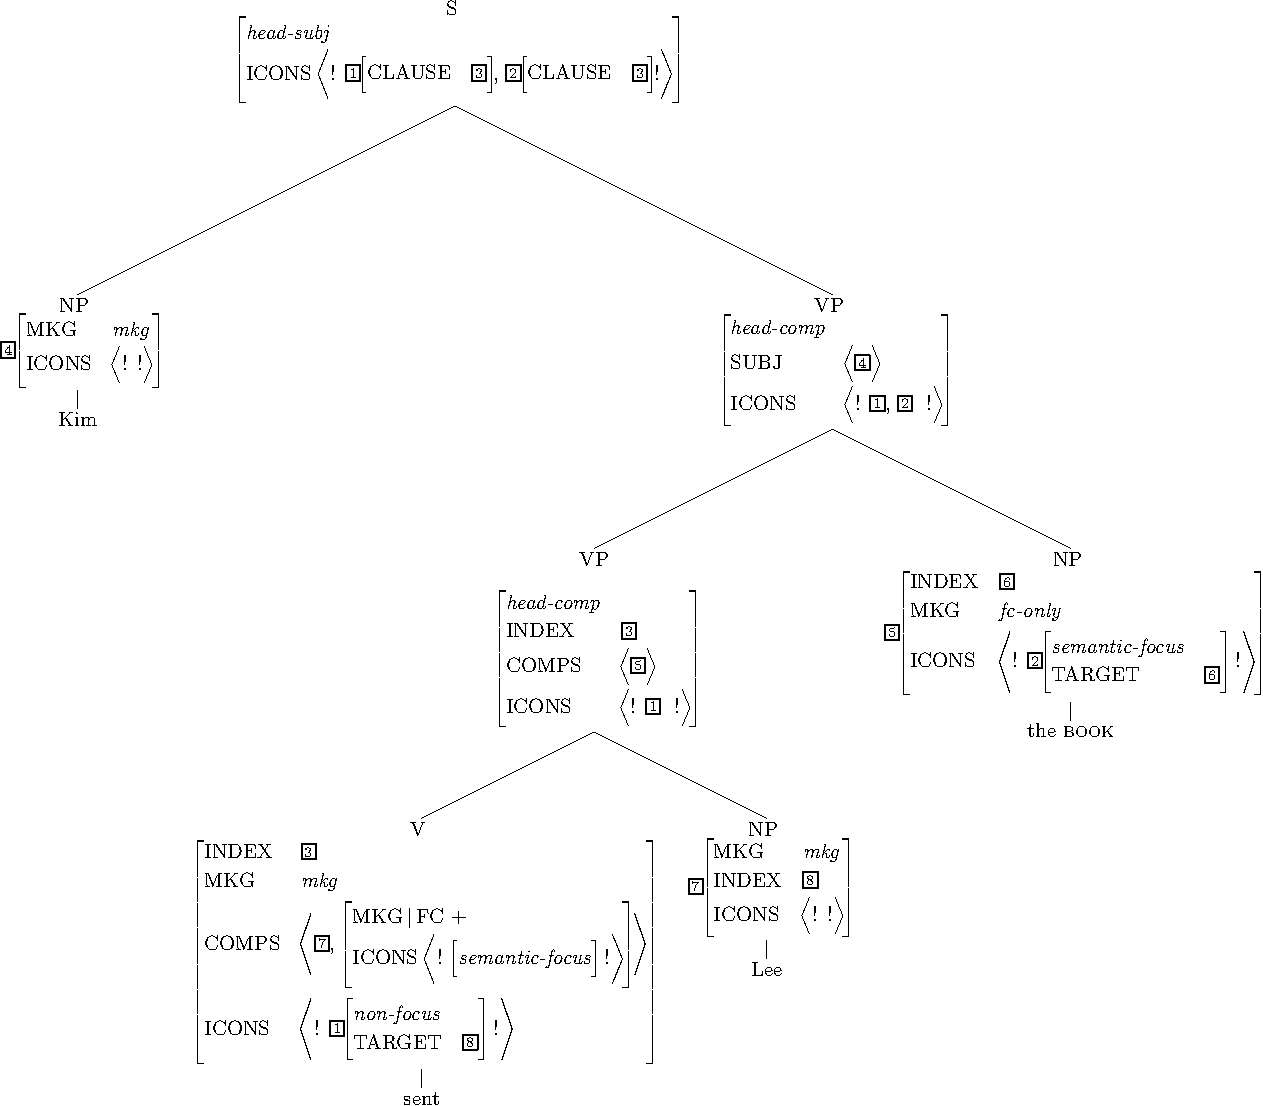
\includegraphics[width=.9\textwidth]{pdf/fp-tree.pdf}}}}


\noindent The corresponding dependency graph is provided
in \myref{fig:fp:graph}. 



\myexe{\enumsentence{\label{fig:fp:graph}\evnup{
      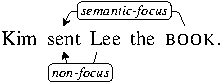
\includegraphics{pdf/fp-graph.pdf}}}}

In \myref{fig:fp:graph}, there are four information structure
relations. Two of them are visible in \myref{fig:fp:graph}: One is
\tdl{non-focus} between \textit{Lee} (unmarked) and the semantic head
\textit{sent}, and the other is the \tdl{semantic-focus} between
\textsc{book} (A-accented) and \tdl{sent}.\is{semantic focus}  In addition to them, there
are two other potential relations, left underspecified in the
dependency graph.  One is between \textit{Kim} and \textit{sent}, and
the other is \textit{sent} to itself. These can be monotonically
specified in further processing. That is, further constraints can be
added, but only if they are consistent with what is there. This
underspecified \isi{ICONS} representation get further specified to VP
\isi{focus} or S focus.\is{underspecification}  According to the graph in \myref{fig:fp:graph},
\textit{Lee} should not be focused, \textit{book} should be focused,
and \textit{Kim} and \textit{sent} may or may not be focused.  When
\textit{sent} is focused, the \isi{ICONS} list in the output includes
three \isi{ICONS} elements (i.e.\ VP focus). When both \textit{sent}
and \textit{sent} are focused, the \isi{ICONS} list in the output
includes four \isi{ICONS} elements (i.e.\ S focus).  When they are
associated with focus, the representations are sketched out in
(\ref{fig:fp:graph:2}a-b), respectively.  Note that the input
representation provided in \myref{fig:fp:graph} subsumes
(\ref{fig:fp:graph:2}a-b), but not \textit{vice versa}.

\myexe{\enumsentence{\label{fig:fp:graph:2}
\begin{tabular}[t]{lllll}
a. & \evnup{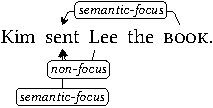
\includegraphics{pdf/fp-graph-v.pdf}} & & b. &
\evnup{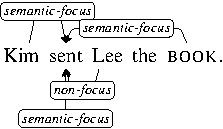
\includegraphics{pdf/fp-graph-s.pdf}} \\
\end{tabular}}}




This representation works especially well in terms of generation.
First, the first element in the final \isi{ICONS} list given in
\myref{fig:fp:tree} assigns \tdl{non-focus} to \textit{Lee}, an
A-accented \textsc{Lee} is ruled out in the generation output.
Second, the second element in the final \isi{ICONS} list assigns
\tdl{semantic-focus} to \textit{the book}, \textit{the book} must be
focus-marked in the generation output (i.e.\ \textit{the
  \textsc{book}}). Third, \textit{Kim} and \textit{sent} in the
underspecified relations can be associated with \tdl{semantic-focus},
and thereby `-a' can be attached to them.  Consequently, the following
three outputs can be generated when using \textit{Kim sent Lee the
  book-a.}  as the input string.  (\ref{exe:fp:gen}a-c) hypothetically
represent NP \isi{focus}, VP focus, and S focus, respectively.\footnote{For
  ease of comparison, the other hypothetical suffix `-b' is not
  considered here.}

\myexe{\enumsentence{\toplabel{exe:fp:gen}
\begin{tabular}[t]{ll}
a. & {Kim sent Lee the book-a.}\\
b. & {Kim sent-a Lee the book-a.}\\
c. & {Kim-a sent-a Lee the book-a.}\\
\end{tabular}}}


Lastly, it is noteworthy that a sentence built with
(\ref{avm:fp:rules}a), such as (\ref{exe:lee:5}a), cannot be further
specified in the same way.  (\ref{avm:fp:rules}a) introduces an
element whose value is \tdl{non-focus} into the \isi{ICONS}
list. Since this constraint prevents the verb \textit{sent} from being
focused, neither VP focus nor S focus can happen in the
sentence. Additionally, since the subject is constrained as [ICONS-KEY
  \tdl{non-focus}] in (\ref{avm:fp:rules}a),\is{ICONS-KEY} an
A-accented \textsc{Kim} cannot be the subject.  In an actual
processing, (\ref{exe:fp:gen:2}a) cannot be paraphrased as sentences
in (\ref{exe:fp:gen:2}b-d).

\myexe{\enumsentence{\toplabel{exe:fp:gen:2}
\begin{tabular}[t]{ll}
a. & {Kim sent Lee-a the book.}\\
b. & {Kim sent-a Lee-a the book.}\\
c. & {Kim-a sent-a Lee-a the book.}\\
d. & {Kim-a sent Lee-a the book.}\\
\end{tabular}}}


\subsection{Further Question}
\label{10-4:ssec:further}

My analysis presented thus far leaves an interesting question for
future work.  The EP that \textit{sent} introduces into the RELS list
is represented as \myref{avm:fp:rels}. In the sentences given in
\myref{exe:lee:5}, the INDEXes of \textit{Kim}, \textit{Lee}, and
\textit{book} have coreferences with ARG1, ARG2, and ARG3,
respectively.


\myexe{\enumsentence{\label{avm:fp:rels}\evnup{
      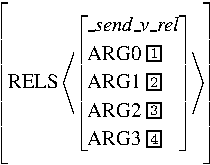
\includegraphics{pdf/fp-rels.pdf}}}}


\noindent In accordance with \myref{avm:fp:rels}, the \isi{ICONS}
lists for (\ref{exe:lee:5}a-b) are constructed as
(\ref{avm:fp:icons:12}a-b).  They explicitly specify the information
structure values on ARG2 and ARG3, but ARG1 is not included in them.



\myexe{\enumsentence{\label{avm:fp:icons:12}
\begin{tabular}[t]{ll}
a. & {Kim sent \textsc{Lee} the book.} \\
   & 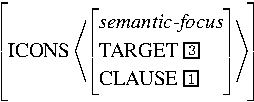
\includegraphics{pdf/fp-icons1.pdf}\\
b. & {Kim sent Lee the \textsc{book}.}\\
   & 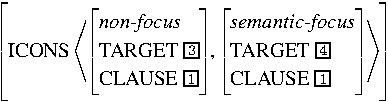
\includegraphics{pdf/fp-icons2.pdf} \\
\end{tabular}}}


The current assumption is that \isi{focus} cannot spread to the role
associated with the subject (here ARG1) without including the
verb.\is{focus projection} For instance, ({\ref{avm:fp:icons:12}b)
  cannot be interpreted in the same way as (\ref{avm:fp:icons:12:2})
  via focus projection, because the \isi{ICONS} in
  (\ref{avm:fp:icons:12:2}) does not contain an element for the
  verb. Note that the first \isi{ICONS} element in
  (\ref{avm:fp:icons:12:2}) is introduced by the A-accent rule for
  \textsc{Kim}.


\myexe{\enumsentence{\label{avm:fp:icons:12:2}
\begin{tabular}[t]{l}
{\textsc{Kim} sent Lee the \textsc{book}.} \\
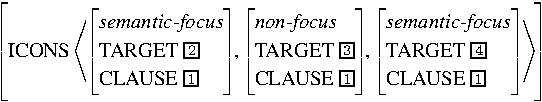
\includegraphics{pdf/fp-icons3.pdf}\\
\end{tabular}}}


This assumption seems linguistically true in that the sentence in
(\ref{avm:fp:icons:12:2}) is not an instance of S focus. The question
is which mechanism technically blocks such specialization. This
mechanism for \isi{focus projection} has to play two functions. First, it
allows the subject (here ARG1) to be associated with focus if and only
if the verb is also associated with focus. Second, it serves to
prevents the \isi{ICONS} list in (\ref{avm:fp:icons:12}a) from being further
specified.  My further research will delve into how the mechanism
works.



\section{Summary}
\label{10-4:sec:sum}

This chapter has offered a new approach of computing focus projection in
terms of sentence generation.\is{focus projection} First, the present
study argues that a single parse tree of a sentence with \isi{focus}
projection is enough to represent the meaning of information structure
and also more effective in the context of \isi{grammar
  engineering}.\is{prosody} Second, F-marking is not necessarily
encoded by prosody. In some languages (e.g.\ Mandarin \ili{Chinese}
and \ili{Korean}), some lexical markers play a role to extend the
domain of focus. Thus, F-marking in the present study is dealt with
[MKG{$\mid$}FC +].\is{MKG} Third, (at least in \ili{English}), focus
projection happens normally when the most peripheral item is
focus-marked though there are some exceptional cases.\is{periphery}
Fourth, there are two more constraints on focus projection. One is
that the the focus-marked element should be included in the focus
domain. The other is that focus-marked elements are preferred to be
headed.\footnote{There are some exceptional cases to this: In the
  sense of entrenched, non-canonical structures, ``languages can
  contain numerous offbeat pieces of syntax with idiosyncratic
  interpretations'' \citep{jackendoff:08}; for example, ``Off with his
  head!'', ``Into the house with you!'', etc.}  In other words, the
focus meaning is seldom extended to any non-head phrases. Building
upon these arguments, the last section in this chapter shows how a
simple ditransitive sentence is analyzed with respect to focus
projection. Two lexical rules are introduced to discriminate a
sentence in which focus projection happens. This is a piece of
evidence to support my argument in this chapter, but a more thorough
study is required in future research.


